\documentclass[a4paper,11pt]{article}
\usepackage[margin=2.5cm]{geometry}
\usepackage{amsmath,amssymb,amsthm}
\usepackage{booktabs}
\usepackage{enumitem}
\usepackage{hyperref}
\usepackage{tikz}

\newtheorem{theorem}{Theorem}
\newtheorem{lemma}[theorem]{Lemma}
\theoremstyle{definition}
\newtheorem{definition}{Definition}

\title{Incremental Rendering of Typeset Documents}
\author{kiwamizamurai}
\date{October 2026}

\begin{document}
\maketitle

\begin{abstract}
We describe a viewer that re-renders Markdown, Typst, and \LaTeX{} documents on every save while preserving the reading position. The design isolates format-specific renderers behind a single interface, so adding a format requires one new implementation and one registration.
\end{abstract}

\tableofcontents

\section{Introduction}
Authors of long documents alternate between editing and reading~\cite{knuth1984}. Systems such as Typst~\cite{madje2023} compile fast enough to make a \emph{save-and-see} loop practical; a viewer need only observe the file system and display the newest output.

\section{Model}
\begin{definition}
A \emph{renderer} is a function $R : \Sigma^{*} \to \mathcal{O}$ from source text to an output $\mathcal{O} = \mathrm{HTML}$.
\end{definition}

\begin{theorem}[Stale results are discarded]\label{thm:stale}
Let renders $r_1, r_2, \ldots$ start at times $t_1 < t_2 < \cdots$. If each carries a monotonically increasing token $k_i$ and only the render with the largest token may update the view, then the displayed output is always $R(s_n)$ for the latest source $s_n$.
\end{theorem}
\begin{proof}
Suppose a render $r_i$ with $i < n$ finishes last. Its token $k_i < k_n$ fails the check, so it is dropped. Hence only $r_n$ can write. \qedhere
\end{proof}

\begin{lemma}\label{lem:sum}
For all $n \ge 1$, $\displaystyle\sum_{k=1}^{n} k = \frac{n(n+1)}{2}$.
\end{lemma}

Combining Theorem~\ref{thm:stale} and Lemma~\ref{lem:sum} is not meaningful, but it exercises cross-references.

\section{Pipeline}
Figure~\ref{fig:pipeline} shows the pipeline, and Table~\ref{tab:formats} lists the converter for each format.

\begin{figure}[h]
\centering
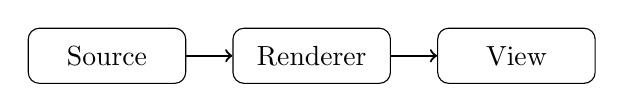
\begin{tikzpicture}[node distance=2.6cm, box/.style={draw, rounded corners, minimum width=2cm, minimum height=7mm}]
  \node[box] (source) {Source};
  \node[box, right of=source] (renderer) {Renderer};
  \node[box, right of=renderer] (view) {View};
  \draw[->, thick] (source) -- (renderer);
  \draw[->, thick] (renderer) -- (view);
\end{tikzpicture}
\caption{The render pipeline.}
\label{fig:pipeline}
\end{figure}

\begin{table}[h]
\centering
\begin{tabular}{@{}ll@{}}
\toprule
Format   & Pipeline            \\
\midrule
Markdown & comrak $\to$ HTML   \\
Typst    & typst $\to$ HTML    \\
\LaTeX{} & pandoc $\to$ HTML   \\
\bottomrule
\end{tabular}
\caption{The converter for each format.}
\label{tab:formats}
\end{table}

\begin{align}
  T_{\text{shown}} &= T_{\text{convert}} + T_{\text{display}} \label{eq:total} \\
  &\ge T_{\text{convert}} \notag
\end{align}

Equation~\eqref{eq:total} splits the time before a document appears into converting and displaying it.

\subsection{Design goals}
\begin{enumerate}[label=(\roman*)]
  \item Keep the scroll position across re-renders.
  \item Surface compiler diagnostics with line and column.
  \item Never execute raw HTML from documents.
\end{enumerate}

\begin{itemize}[nosep]
  \item Formats are added by implementing one trait.
  \item External engines are injected for testing.
\end{itemize}

\section{Conclusion}
A small, well-factored viewer is sufficient for a fast save-and-see loop.

\bibliographystyle{plain}
\bibliography{refs}

\end{document}
